\documentclass[10pt]{beamer}

% Font and language setup (XeLaTeX / LuaLaTeX compatible)
\usepackage{fontspec}
\setsansfont{Arial}
\setmainfont{Times New Roman}
\usepackage[english,greek]{babel} % Greek is the main/default language

\usepackage{booktabs}
\usepackage{graphicx}
\usepackage{amsmath}
\usepackage{tikz}

% Modern Blue & White Palette Settings
\definecolor{primaryblue}{RGB}{20, 60, 110}   % Deep corporate blue
\definecolor{secondaryblue}{RGB}{60, 110, 170} % Medium accent blue
\definecolor{lightblue}{RGB}{235, 243, 250}    % Soft blue background for blocks
\definecolor{darkgray}{RGB}{40, 40, 40}        % Neutral dark for text

\usetheme{Madrid}
\usecolortheme{default}

% Override colors for standard Beamer elements
\setbeamercolor{structure}{fg=primaryblue}
\setbeamercolor{palette primary}{bg=primaryblue,fg=white}
\setbeamercolor{palette secondary}{bg=secondaryblue,fg=white}
\setbeamercolor{palette tertiary}{bg=primaryblue!80!black,fg=white}
\setbeamercolor{palette quaternary}{bg=primaryblue!60!black,fg=white}
\setbeamercolor{titlelike}{parent=palette primary,fg=white}
\setbeamercolor{block title}{bg=primaryblue,fg=white}
\setbeamercolor{block body}{bg=lightblue,fg=darkgray}

% Customize itemize bullets
\setbeamertemplate{itemize items}[circle]

% Turn off navigation symbols for a cleaner look
\setbeamertemplate{navigation symbols}{}

\title[Safe Mobile Robot Navigation]{Safe Mobile Robot Button Navigation}
\subtitle{(Ομάδα 1)}
\author[Ε.Π. \& Δ.Φ.]{Εμμανουήλ Παξιμαδάκης (1100972) \\ Δημήτριος Φιλόπουλος (1101130)}
\institute[Παν. Πατρών]{Τμήμα Ηλεκτρολόγων Μηχανικών \& Τεχνολογίας Υπολογιστών \\ Πανεπιστήμιο Πατρών}
\date[Ιούνιος 2026]{29 Ιουνίου 2026}

\begin{document}

% Slide 1: Title
\begin{frame}
    \titlepage
\end{frame}

% Slide 2: Goal & Environment
\begin{frame}{2. Στόχος \& Περιβάλλον Προσομοίωσης}
    \begin{block}{Ορισμός του Προβλήματος}
        Σχεδιασμός ενός navigation controller για ένα αυτόνομο όχημα \textbf{Racecar} στο περιβάλλον \texttt{SafetyRacecarButton2-v0} της \textbf{Safety Gymnasium}.
    \end{block}
    
    \begin{columns}
        \begin{column}{0.4\textwidth}
            \begin{figure}
                \centering
                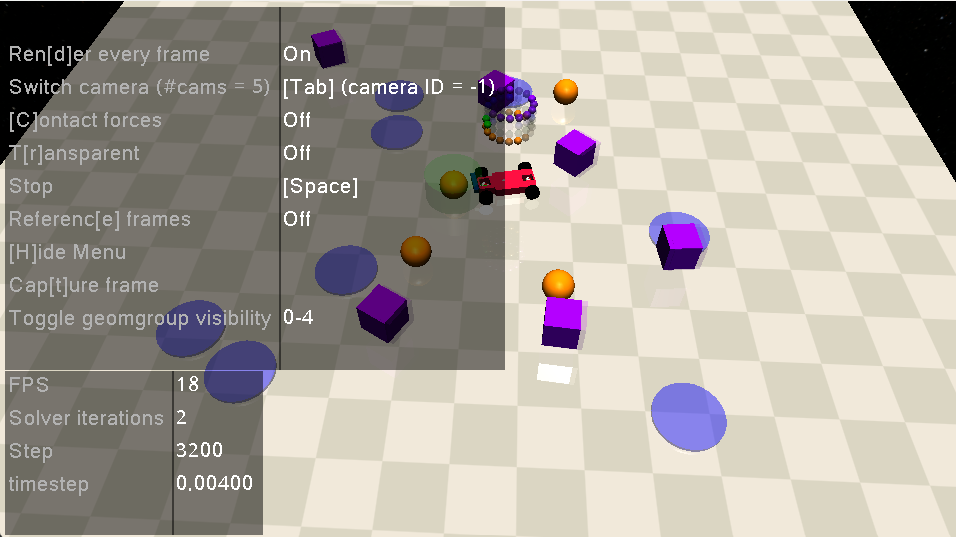
\includegraphics[width=\linewidth]{safety_gymnasium.png}
                \caption{Περιβάλλον Racecar}
            \end{figure}
        \end{column}
    \end{columns}
\end{frame}

% Slide 3: Preprocessing and Wrappers
\begin{frame}{3. Προεπεξεργασία και Wrappers}
    Για τη σταθεροποίηση της εκπαίδευσης και τη βελτιστοποίηση της κίνησης του ρομπότ εφαρμόστηκαν:
    
    \vspace{0.2cm}
    \begin{enumerate}
        \item \textbf{Action Smoothing (EMA):} 
        Αποτρέπει απότομες αλλαγές πορείας και προστατεύει από drifting: 
        \[a_{t,\text{smooth}} = \alpha \cdot a_t + (1 - \alpha) \cdot a_{t-1,\text{smooth}}\]
        
        \item \textbf{Observation Normalization (Welford)}
        \item \textbf{Lagrangian Shaped Reward:}
        Ανταμοιβή με βάση το τρέχον κόστος:
        \[ r_{t,\text{shaped}} = r_t - \beta \cdot c_t \]
    \end{enumerate}
\end{frame}

% Slide 4: The 3 Controllers
\begin{frame}{4. Controllers}
    \begin{columns}[t]
        \begin{column}{0.32\textwidth}
            \begin{block}{Scripted Controller}
                \small
                \textbf{Rule-Based}
                \begin{itemize}
                    \item Heuristic λήψη αποφάσεων βάσει Lidar.
                    \item Gear selection ανάλογα με τη γωνία του στόχου.
                    \item Απότομη στροφή/επιβράδυνση κοντά σε εμπόδια.
                    \newline
                \end{itemize}
            \end{block}
        \end{column}
        
        \begin{column}{0.32\textwidth}
            \begin{block}{Simple PPO}
                \small
                \textbf{Reward-Only}
                \begin{itemize}
                    \item Εκπαίδευση με Proximal Policy Optimization.
                    \item Αγνοεί πλήρως το κόστος ασφάλειας ($c_t$).
                    \item Επιθετική οδήγηση με στόχο μόνο τα buttons.
                    \newline
                    \newline
                \end{itemize}
            \end{block}
        \end{column}
        
        \begin{column}{0.32\textwidth}
            \begin{block}{PPO-Lagrangian}
                \small
                \textbf{Constrained RL}
                \begin{itemize}
                    \item Βελτιστοποίηση Reward με Όρια Ασφάλειας
                    \item Δυναμικός πολλαπλασιαστής Lagrange $\beta$ με gradient ascent.
                    \item Εξισορροπεί αυτόματα πλοήγηση και ασφάλεια.
                \end{itemize}
            \end{block}
        \end{column}
    \end{columns}
\end{frame}


% Slide 8: Conclusions & Comparison
\begin{frame}{5. Συμπεράσματα \& Συγκριτική Ανάλυση}
    \begin{table}
        \small
        \centering
        \begin{tabular}{lcccc}
            \toprule
            \textbf{Ελεγκτής} & \textbf{Reward ($R$)} & \textbf{Cost ($C$)} & \textbf{Zero-Cost \%} & \textbf{Combined Score} \\
            \midrule
            Scripted & \textbf{+3.14} & 202.80 & 10.0\% & -199.66 \\
            Simple PPO & +2.82 & 170.85 & 15.0\% & -168.03 \\
            \textbf{PPO-Lagrangian} & +1.29 & \textbf{136.10} & \textbf{30.0\%} & \textbf{-134.81} \\
            \bottomrule
        \end{tabular}
        \caption{Συγκριτικός Πίνακας Επιδόσεων}
    \end{table}
    
 
\end{frame}

% Slide 6: Future Work (Behavioral Cloning & Pre-training)
\begin{frame}{6. Μελλοντικές Βελτιώσεις}
	\begin{block}{}
		Συνδυασμός της \textbf{Heuristic λογικής} (Scripted Controller) με την \textbf{Ενισχυτική Μάθηση} (PPO-Lagrangian).
	\end{block}
	
	\textbf{Υλοποίηση:}
	\begin{enumerate}
		\item \textbf{Behavioral Cloning:} 
		Εκπαίδευση της policy με Supervised Learning πάνω στον Scripted Controller
		\item \textbf{RL Fine-Tuning:} 
		Με χρήση του PPO-Lagrangian.
	\end{enumerate}
	
	\vspace{0.2cm}
	\textbf{Αναμενόμενα Οφέλη:}
	\begin{itemize}
		\item \textbf{Ταχύτερη Σύγκλιση}
		\item \textbf{Ασφαλέστερη Εκπαίδευση}
	\end{itemize}
\end{frame}

\end{document}
